%%%%%%%%%%%%%%%%%%%%%%%%%%%%%%%%%%%%%%%%%%%%%%%%%%%%%%%%%%%%%%%%%%%%%%%%%%%%%%%%%%%%%
%																					%
%	TRABAJO: Proyecto Integrador													%
%																					%
%		Titulo: 	Desarrollo de IP cores con procesamiento de Redes de Petri 		%
%					Temporales para sistemas multicore en FPGA						%
%																					%
%		Autores:	Juli�n Nonino													%
%					Carlos Renzo Pisetta											%
%		Director:	Orlando Micolini												%
%																					%
%	Parte: Desarrollo																%
%	Capitulo: Dise�o e Implementaci�n												%
%	Seccion: Arquitectura general del sistema										%	
%	Archivo: arquitectura_general.tex												%
%																					%
%%%%%%%%%%%%%%%%%%%%%%%%%%%%%%%%%%%%%%%%%%%%%%%%%%%%%%%%%%%%%%%%%%%%%%%%%%%%%%%%%%%%%

% Path Imagenes: ./desarrollo/diseno_implementacion/img
% Nombre predeterminado imagenes: disenoxx
%	xx es el numero de imagen

\section{Arquitectura general del sistema}
	\label{sec:arquitectura_general}

	Al comenzar el trabajo, se creo un esquema para describir la ubicaci�n y la conexi�n
	del procesador de Petri en un sistema multicore.
	\begin{figure}[ht]
		\centering
		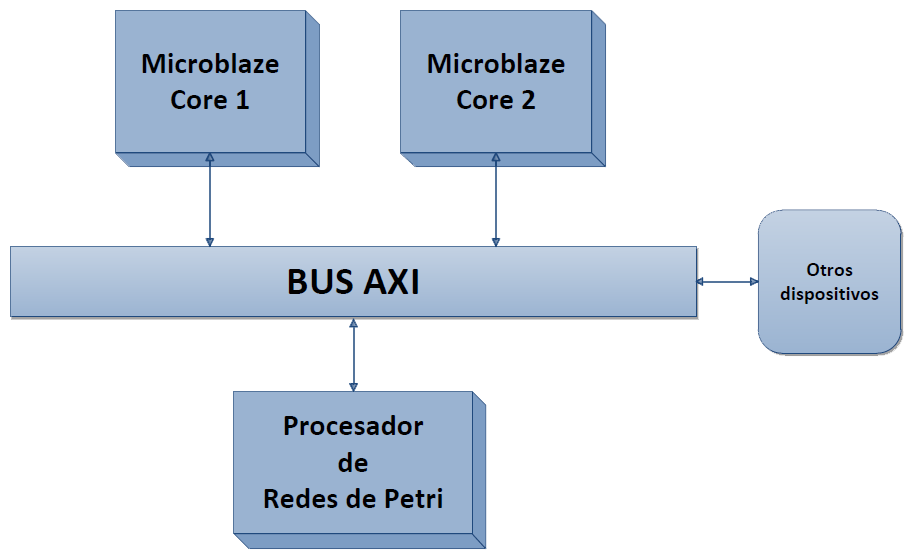
\includegraphics[width=1\linewidth,keepaspectratio]{./desarrollo/diseno_implementacion/img/diseno01}
		\caption{Arquitectura general del sistema}
		\label{fig:diseno01}
	\end{figure}
	
	En el diagrama de la \ref{fig:diseno01}, se observa como esta ubicado el procesador 
	de Petri dentro del sistema. Existen dos cores MicroBlaze de Xilinx que a trav�s del BUS 
	AXI se comunicaran con el procesador de Petri para sincronizarse.
	Se plante� un sistema con dos procesadores ya que este es el m�nimo numero de cores para 
	que el sistema sea multicore.
	El procesador de Redes de Petri se encuentra conectado al bus AXI independientemente de 
	los otros procesadores del sistema porque de esta forma, la �nica limitaci�n en el acceso 
	al procesador de Redes de Petri ser�a el bus.